\documentclass[a4paper,zihao=5,UTF8]{ctexart}
\usepackage[top=2.3cm,bottom=2cm,left=1.7cm,right=1.7cm]{geometry} 
\usepackage{amsmath, amssymb}
\usepackage{color}
\usepackage{hyperref} 
\usepackage{pythonhighlight}
\usepackage{listings}
\usepackage{mathrsfs} 
\usepackage{booktabs}
\usepackage{amsthm}
\usepackage{longtable} 
\usepackage{graphicx}
\usepackage{subfigure}
\usepackage{caption}
\usepackage{fontspec}
\usepackage{titlesec}
\usepackage{fancyhdr}
\usepackage{latexsym}
\usepackage{subfigure}
\usepackage{braket}
\usepackage{cite}
\usepackage[version=4]{mhchem}
\usepackage{makecell}

\CTEXsetup[format={\Large\bfseries}]{section}
\def\d{\mathrm{d}}
\def\e{\mathrm{e}}
\def\i{\mathrm{i}}
\def\dps{\displaystyle}
\newcommand{\mr}[1]{\mathrm{#1}}
\newcommand{\mb}[1]{\mathbf{#1}}
\newcommand{\dv}[2]{\frac{\d{#1}}{\d{#2}}}
\newcommand{\pdv}[2]{\frac{\partial{#1}}{\partial{#2}}}
\def\degree{$^{\circ}$}
\def\celsius{^{\circ}\mr{C}}
\title{\textbf{实验七 醋酸亚铬二水合物的合成与表征}\cite{inorganic_chemistry_1}}
\author{王崇斌\;1800011716}
\makeatletter
\makeatother
\begin{document}
	\pagestyle{fancy}
	\pagestyle{fancy}
    \lhead{无机化学实验}
	\chead{}
	\rhead{\today}
	\maketitle
    \thispagestyle{fancy}
    \section{实验目的}
    \begin{enumerate}
        \item 合成醋酸亚铬水合物,学习无氧合成技术
        \item 测定醋酸亚铬水合物的磁化率,了解物质的磁性
        \item 了解醋酸亚铬水合物中多重金属键的成键和结构特征
    \end{enumerate}
    \section{实验原理}
        \subsection{磁化率与分子磁矩}
        对于单个原子而言,其磁性主要来源于基态的角动量(轨道角动量和自旋角动量),
        原子的轨道角动量与自旋角动量会与外加的电磁场相互作用,使得原有的原子能级
        发生偏移(可以将外场看作对于原本体系的微扰)
        \footnote{
            稍微详细地讨论一下单个原子在外磁场中的行为,一般来说,在外磁场中(假设
            外磁场朝向z方向)原子的哈密顿量可以写为(Gauss单位制):
            \begin{equation}
                \hat{H} = \sum_{i=1}^{N_e}\frac{\hat{\mb{p}_{i}}^2}{2m_e}
                + \hat{U}(\{\vec{r}_i\}) + \mu_B\hat{\mb{L}}\cdot\mb{H}
                + \frac{e^2}{8m_ec^2}H^2\cdot\sum_{i=1}^{N_e}(x_{i}^2 + y_i^{2})
                + g_0\mu_BH\hat{S}_z
            \end{equation}
            其中前两项为原子本身的哈密顿量,后面为磁场附加的哈密顿量,如果考虑使用
            定态微扰计算能级的偏移,在仅保留到二阶微扰同时保留$H^2$量级的项时,能级n的
            偏移可以表示为:
            \begin{equation}
                \Delta E_n = \mu_B\mb{H}\cdot\braket{n|\hat{\mb{L}} + g_0\hat{\mb{S}}|n}
                + \sum_{n'\neq n}\frac{\left|\braket{n|\mu_B\mb{H}\cdot(\hat{\mb{L}} + g_0\hat{\mb{S}})|n'}\right|^2}{E_n - E_{n'}}
                + \frac{e^2}{8m_ec^2}H^2\braket{n|\sum_{i=1}^{N_e}(x_i^2+y_i^2)|n}
            \end{equation}
            其中第一项(Zeeman效应)对于能量的贡献是显著的,也是一般顺磁固体所
            表现的顺磁性的来源。第二项只有在基态角动量等于0时有贡献,表现出顺磁性
            (Van Vleck paramagnetism)。最后一项表现出抗磁性(Larmor diamagnetism),
            对于任意的含有闭壳层原子实的原子,此项都会贡献抗磁性,但是其量级远小于
            Zeeman spliting导致的顺磁性,这一项也是闭壳层原子(或者说电子自旋
            配对)组成的材料显示出很弱的抗磁性的原因。\cite{solid_state_physics}
        }
        ,能级变化可以看作原子被磁化。
        \par 
        对于一般的宏观物体,讨论其磁性
        就要考虑系统在有限温度下在不同能级上的分布。对于最简单的情况,如果认为
        各个磁性原子之间没有比较强的相互作用
        (对于磁性原子比较稀疏的顺磁固体,这种近似是合适的)
        ,可以认为是近独立子系,那么系统
        的总磁化强度可以表示为单个原子磁化强度之和:
        \begin{equation}
            M = -\frac{N}{V}\pdv{f}{H}
        \end{equation}
        其中$f$为单原子的自由能(获得了原子能级在外场下的分裂之后
        就可以给出)
        \footnote{
            考虑角动量不为0的原子,假设其基态总角动量($\hat{\mb{J}}:=\hat{\mb{L}} + \hat{\mb{S}}$)
            量子数为J(可以根据Hund规则确定一般的原子的基态角动量情况),
            只考虑Zeeman spliting的贡献,能级可以写为:
            \begin{equation}
                \Delta E(J_z) = \mu_B\mb{H}\cdot\braket{0|\hat{\mb{L}} + g_0\hat{\mb{S}}|0} = g(JLS)\mu_B HJ_z
            \end{equation}
            这一步用到了Wigner-Eckart定理,$g(JLS)$是一个与角动量耦合态的量子数有关的函数,
            这里不再显式给出。那么正则配分函数可以写为:
            \begin{equation}
                z = \e^{-\beta f} = \sum_{J_z = -J}^{J}\e^{-\beta g(JLS)\mu_BHJ_z}
            \end{equation}
            上式可以由等比数列求和给出解析表达式,这里不再给出。
        }
        ,$N,V$分别为磁性原子数目和总体积。
        那么体积磁化率可以表示为:
        \begin{equation}
            \kappa = -\frac{N}{V}\pdv{^2f}{H^2}
        \end{equation}
        由实验讲义上的定义,比磁化率和摩尔磁化率为:
        \begin{equation}
            \begin{split}
            \chi &= \frac{\kappa}{\rho}\\
            \chi_{m} &= \frac{\kappa}{\rho}M
            \end{split}
        \end{equation}
        \par 
        对于顺磁固体(其顺磁性主要由基态角动量不为零的磁性原子贡献),其摩尔磁化率
        在温度较高时可以用\textbf{居里定律}
        \footnote{
            事实上,居里定律可以从在高温极限下近似注释[2]中的配分函数得到
        }
        描述(国际单位制):
        \begin{equation}
            \chi_{m,p} = \frac{N_A\mu_{m}^2\mu_0}{3k_B T}
        \end{equation}
        \par 
        这里给出国际单位制下单电子数目的计算公式(后面给出的标样磁化率是国际单位制下的):
        \begin{equation}
            n = \sqrt{1 + 797.2\chi_m T} - 1
        \end{equation}
        \subsection{磁化率的测量}
        磁化率的测量依靠Gouy磁天平的方法。利用了磁矩在非均匀外场中会受力这一特点,
        测定样品在非匀强磁场中的“质量差”来计算出受力大小,进一步推算出样品磁矩。
        如果假设磁场中心处场强为$H$,磁场边缘处场强为$H_0$,其间磁场线性变化,那么
        可以推算出样品收到磁场作用力为
        \footnote{
            利用磁场中磁矩的能量公式:
            \begin{equation}
                U = \int\kappa B\d V
            \end{equation}
            与受力公式:
            \begin{equation}
                \mb{F} = -\nabla U
            \end{equation}
            可以计算得到。
        }
        :
        \begin{equation}
            F = -\frac{1}{2}(\kappa - \kappa_0)A(H^2 - H_0^2)
        \end{equation}
        其中$A$为平行于磁场方向的样品的截面积。
        \par 
        利用标准物质(莫尔盐)标定,同时通过测定空管的质量读数变化,扣除
        空管抗磁性的影响的方法,可以得到最终样品摩尔磁化率的计算公式:
        \begin{equation}
            \chi_{m,sample} = \chi_{standard}M_{sample}\frac{m_{standard}(\Delta m_{sample} - \Delta m_{0})}
            {m_{sample}(\Delta m_{standard} - \Delta m_{0})}
        \end{equation}
        其中$\Delta m$表示有磁场和无磁场时天平读数的变化,$\chi_{standard}$为标准样品
        比磁化率。
        \subsection{醋酸亚铬二水合物与金属-金属多重键}
        \ce{Cr_2(OOCCH_3)_4(H_2O)_2},是一种深红色晶体。该化合物中含有Cr-Cr键,
        键长为236pm,远远短于金属铬中的Cr-Cr距离249pm。一般认为其中形成了金属-金属四重键,
        由于电子全部成对,理论上它是反磁性的物质。
        \begin{figure}[htbp]
            \centering
            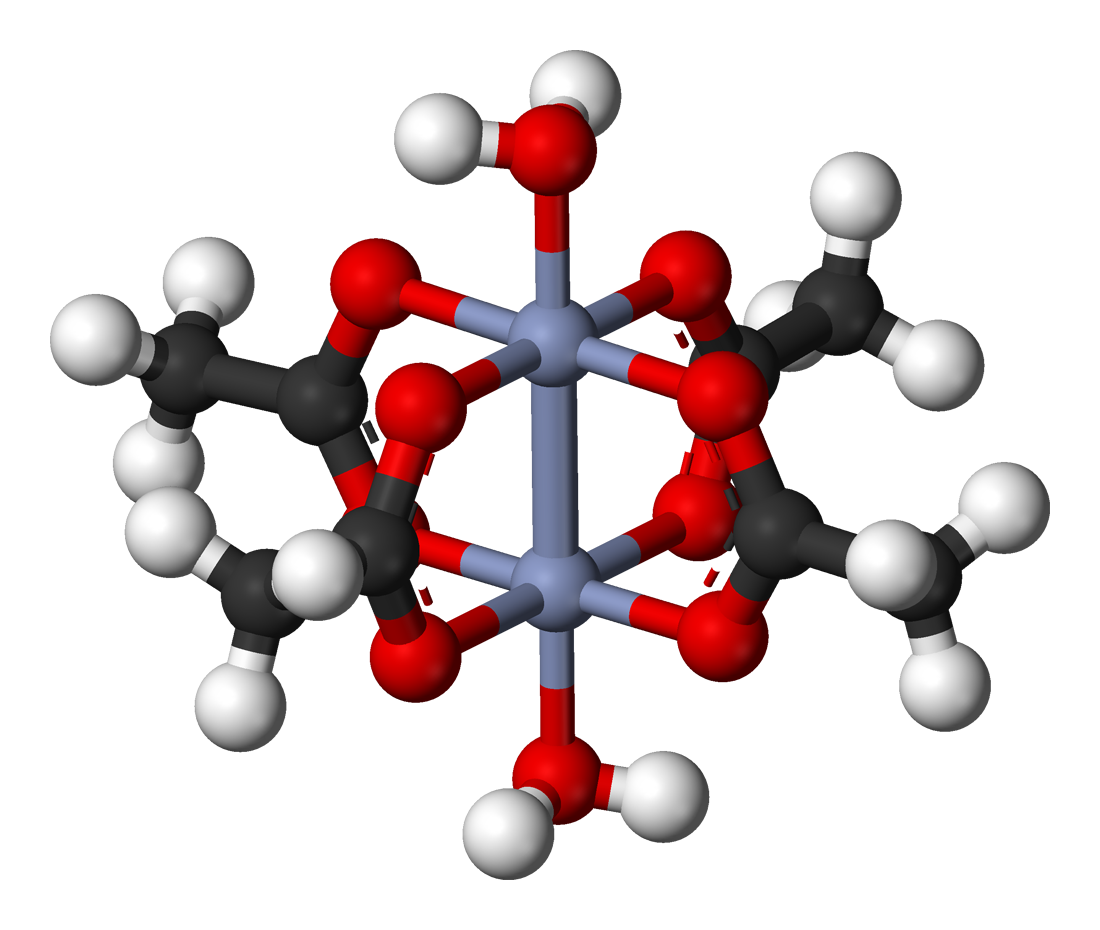
\includegraphics[scale=0.15]{Chromium(II)-acetate-dimer-3D-balls.png}
            \caption{醋酸亚铬水合物的结构示意图}
        \end{figure}
        \begin{figure}[htbp]
            \centering
            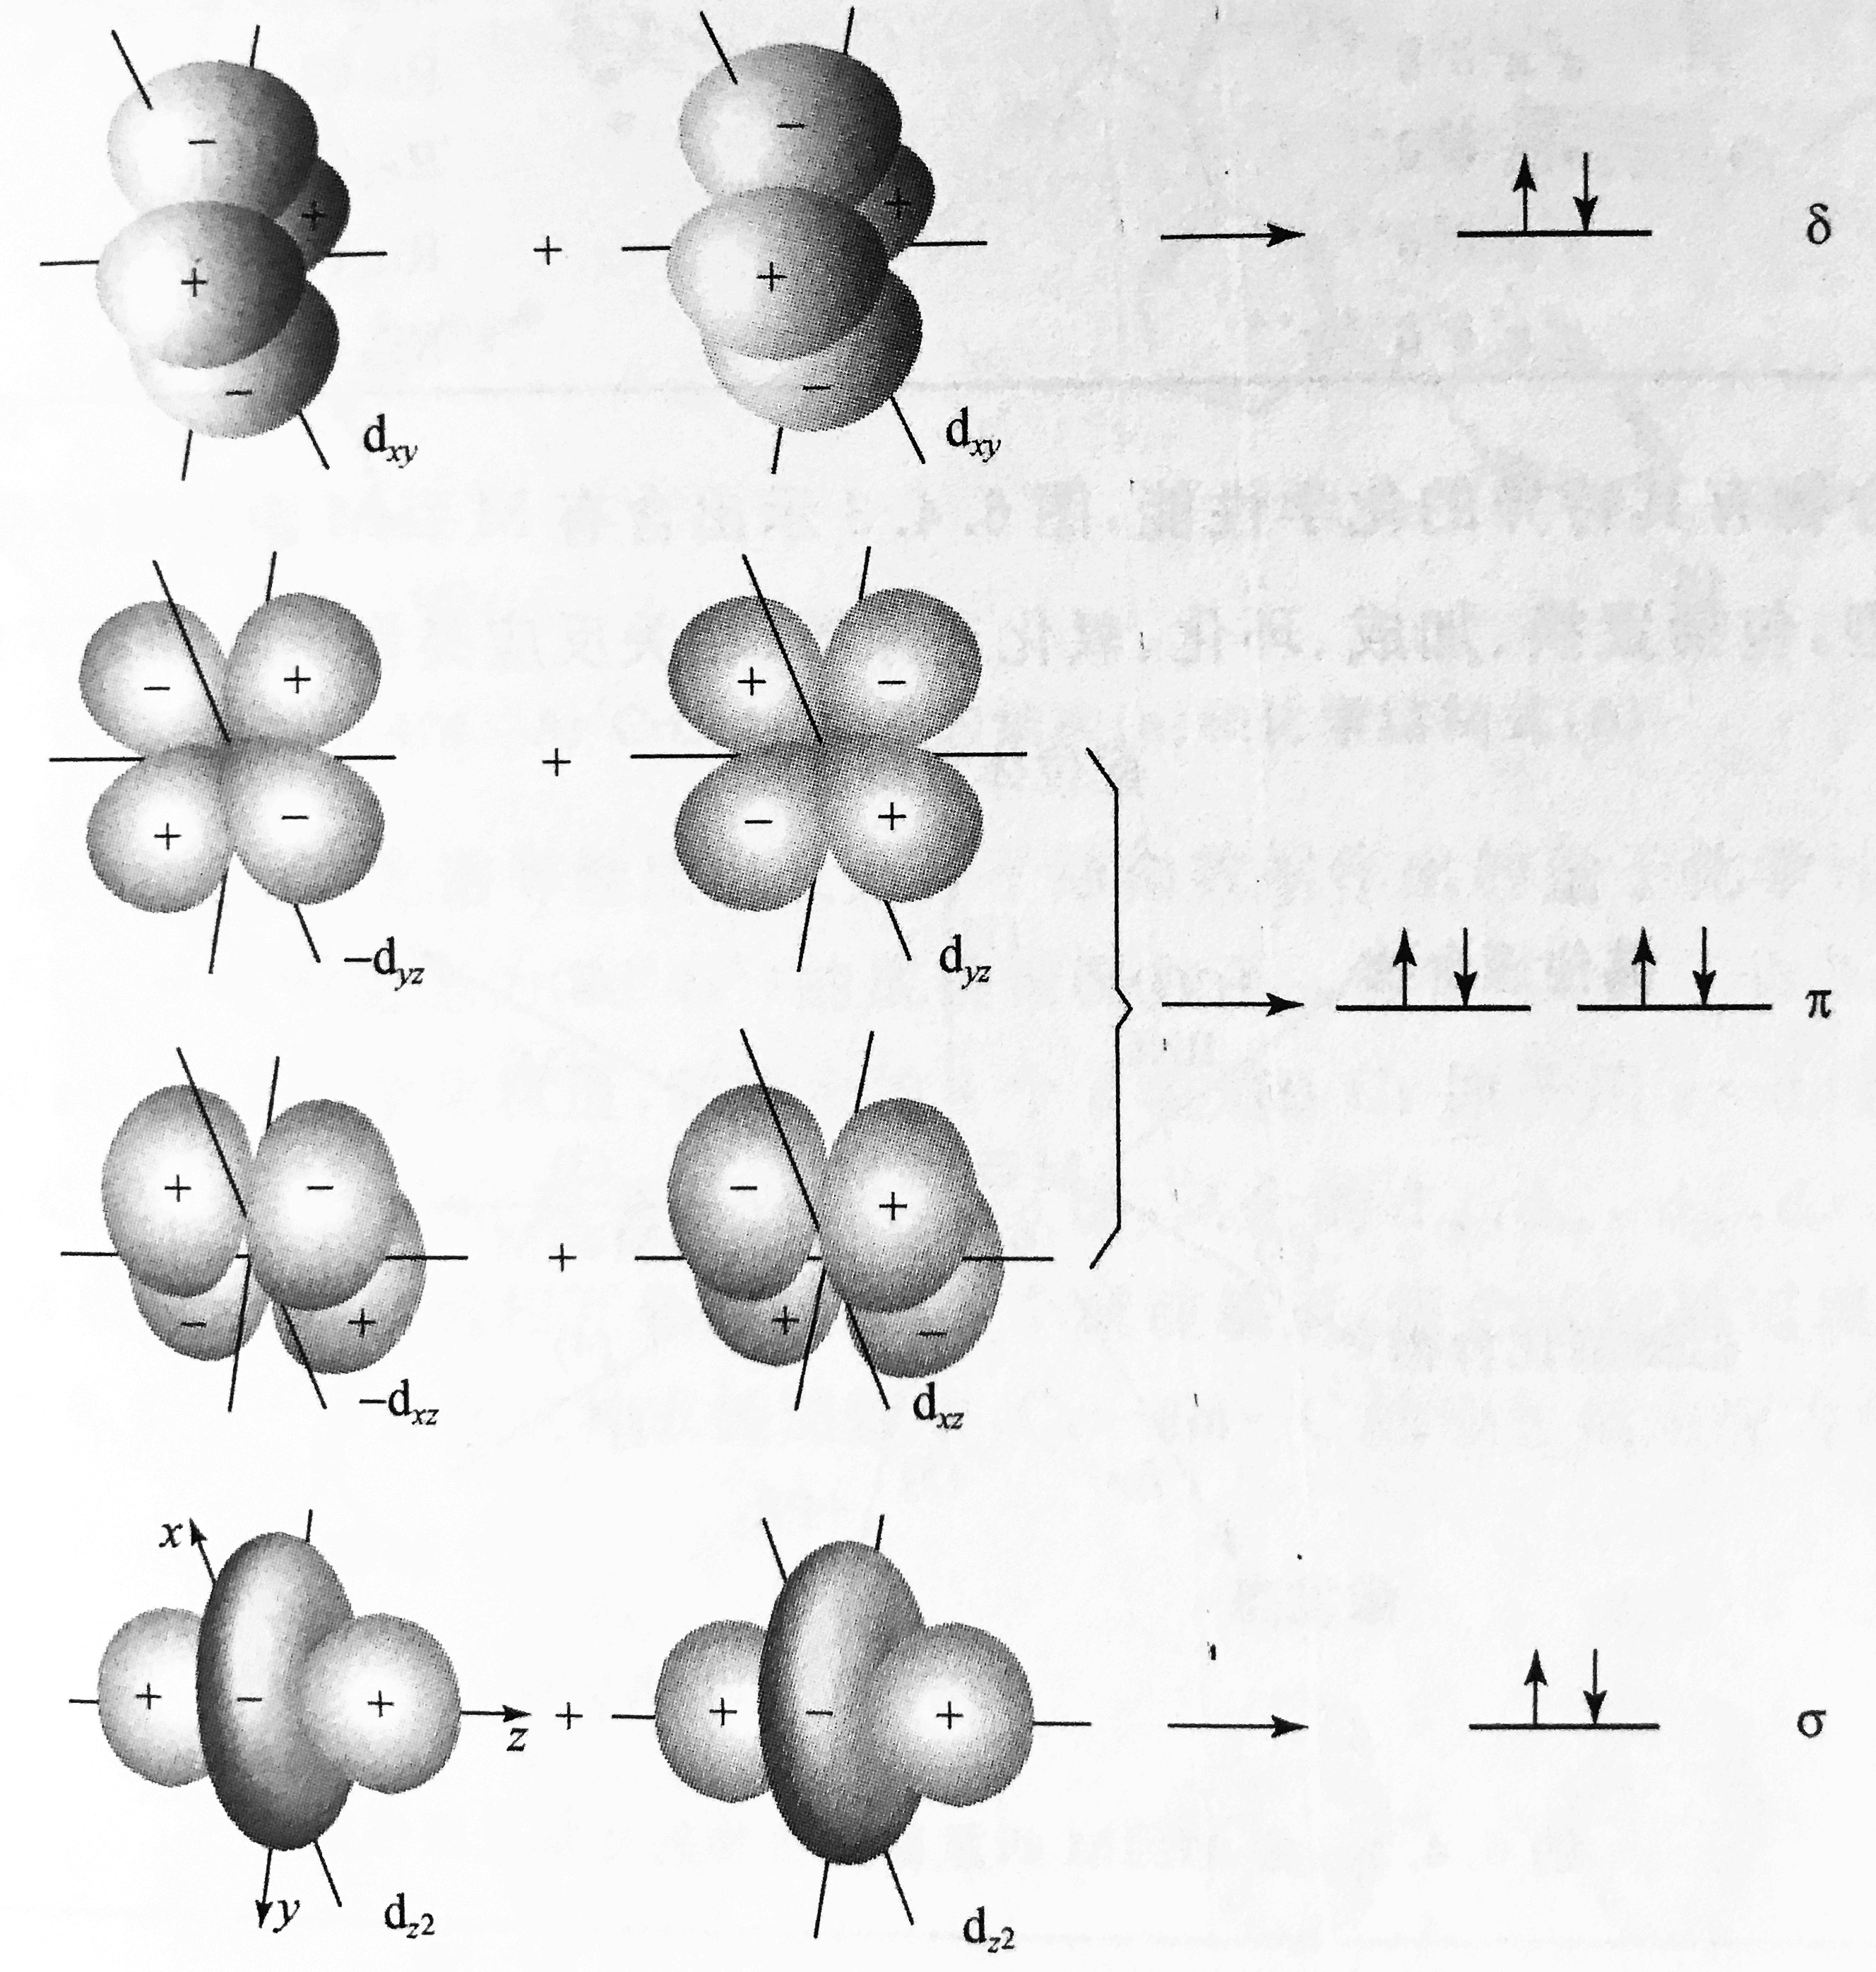
\includegraphics[scale=0.06]{delta_bond.jpg}
            \caption{醋酸亚铬水合物中金属键的成键示意图}
        \end{figure}
        \par 
        它是最稳定的二价铬化合物之一,但在潮湿的情况下极易被空气氧化,所以需要在隔绝
        空气的环境中还原\ce{Cr(III)}溶液制备,同时干燥的那一步要彻底。
        \section{实验步骤与实验现象}
        \begin{enumerate}
            \item 实验地点:北京大学化学与分子工程学院D区三层第七实验室2号实验台
            \item 实验时间:2021年5月21日星期五
        \end{enumerate}
        \subsection{\ce{CrCl_2}的合成}
        按照图\ref{zhuangzhi}接好反应装置,检查装置的气密性(用手捂热观察是否
        有气泡冒出)。称取3.84g,14.4mmol(3.86g,14.5mmol)\ce{CrCl_{3}.6H_2O}
        溶解于6ml去离子水中。称取3.6g(3.59g) Zn粒,将其与搅拌子一起加入反应瓶1中,随后用
        长颈漏斗将氯化铬溶液加入到反应瓶1中,注意不要将液体溅到瓶壁上。
        \par 
        在1.8ml浓盐酸与20ml去离子水的混合溶液中,搅拌下加入12.6g(12.63g)无水醋酸钠
        至大部分溶解,而后将溶液转移入反应瓶6中,在其中加入一个搅拌子。
        \par 
        取4.8ml浓盐酸加入恒压滴液漏斗2中,在气袋3中充好\ce{N_2},将其接在二通活塞4的位置,
        将反应瓶6放置于一个大烧杯中(方便后面水浴加热)。关闭全部二通活塞,打开水泵,同时
        打开二通活塞7,抽去体系内空气(氧气),观察滴液漏斗内的盐酸,当其中由气泡冒出时立刻停止
        抽气,关闭7打开4让氮气进入体系。如此反复3次,体系内的氧气含量降至1\%之下。关闭
        反应装置的所有活塞
        \par 
        此时在活塞7处连接上橡皮管,做好水封,打开4处活塞,用力挤压气袋3,此时打开活塞7,排出橡皮管
        内的空气。之后关闭7与4,倾斜恒压滴液漏斗,打开漏斗的活塞,放入约$\frac{1}{4}$体积的浓盐酸,
        同时迅速打开7,可以观察到水封处由气泡冒出。后续的操作与过程见表\ref{xianxiang}。
        \begin{table}[htbp]
            \centering 
            \caption{加入浓盐酸的时间与实验现象}
            \begin{tabular}[htbp]{ccc}
                \toprule
                时间 & 操作 & 现象 \\
                \midrule
                13:30 & 加入$\frac{1}{4}$浓盐酸 & 溶液深绿色,有气泡产生\\
                13:35 & 加入$\frac{1}{4}$浓盐酸 & 溶液变为青色\\
                13:40 & 加入$\frac{1}{4}$浓盐酸 & 溶液变为蓝绿色,明显放热\\
                13:45 & 加入$\frac{1}{4}$浓盐酸 & 溶液变为蓝色\\
                13:50 & 无 & 溶液为亮蓝色,锌粒未消耗完,溶液很烫\\
                \bottomrule
            \end{tabular}
            \label{xianxiang}
        \end{table}
        \begin{figure}
            \centering
            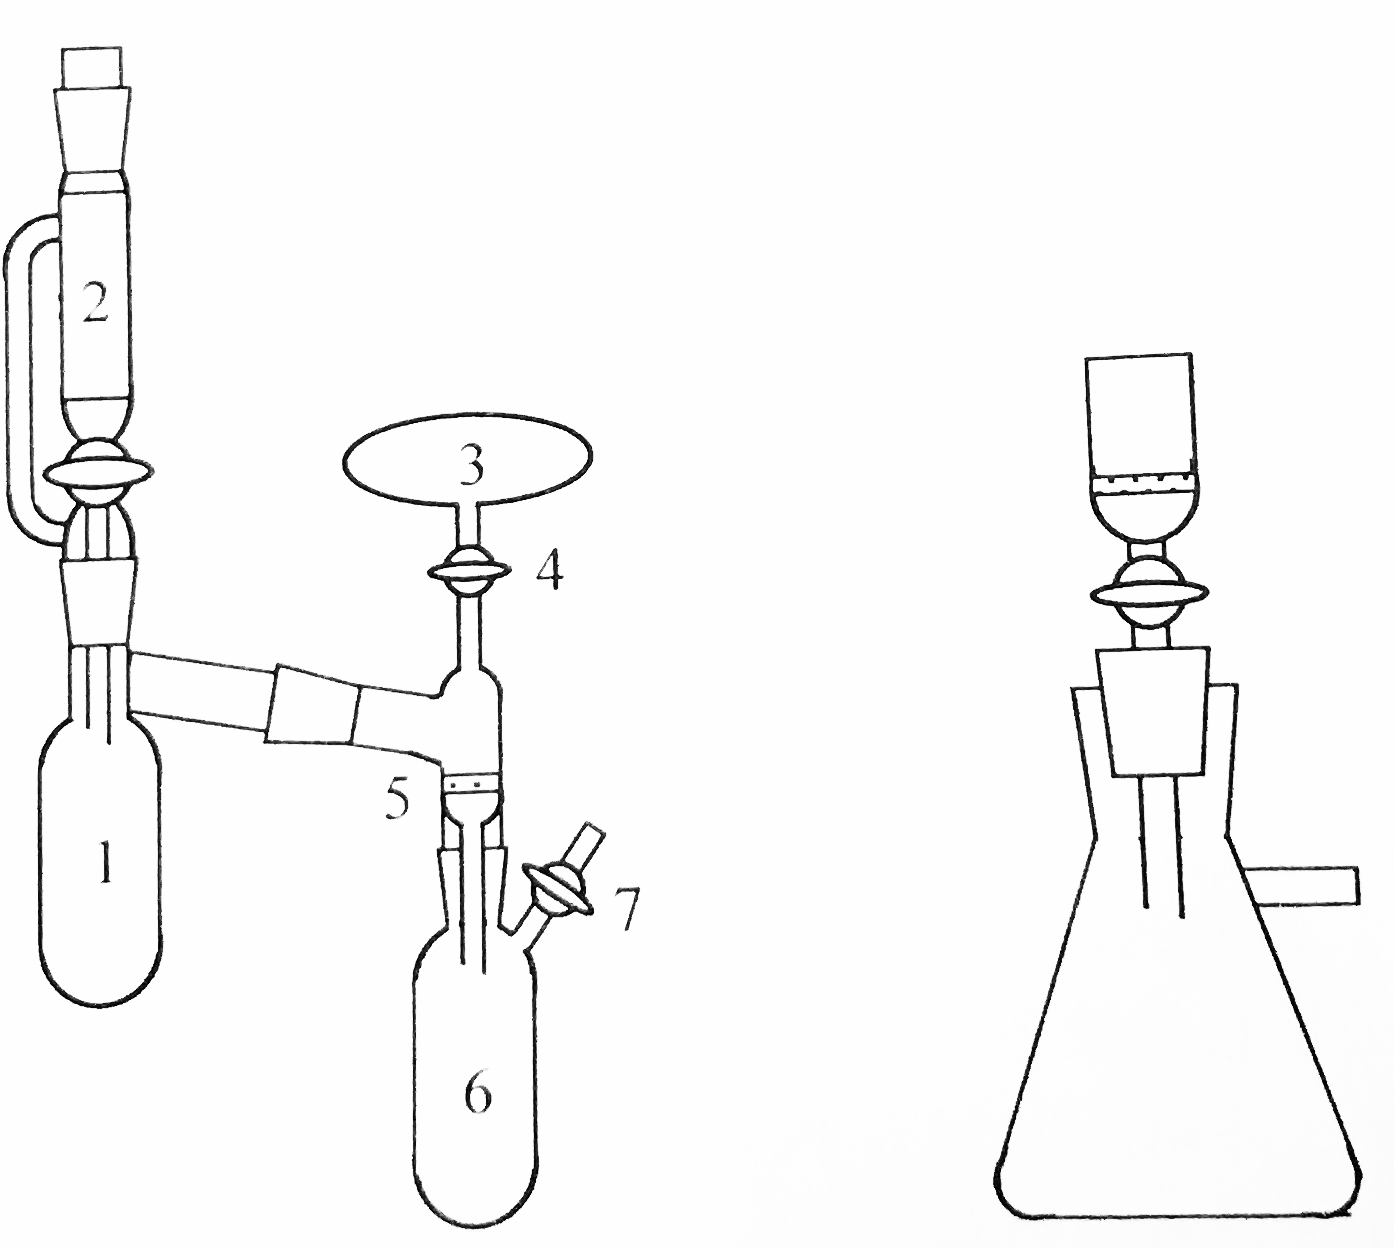
\includegraphics[scale=0.13]{zhuangzhi.jpg}
            \caption{反应装置示意图}
            \label{zhuangzhi}
        \end{figure}
        \subsection{醋酸亚铬水合物的合成}
        当步骤1快结束之前,将接近沸腾的热水倒入装在反应瓶6的大烧杯中,当反应1结束后,
        立即将磁力加热搅拌器移动到6的下方,开启加热。转动反应瓶1使亚铬溶液通过玻璃砂板
        5滴入6中(控制滴入速度不要太快),滴入的溶液会以紫红色的颜色扩散,当滴入足够多后
        6底部开始聚集深红色结晶状固体。加入完毕后停止加热,开动搅拌1min,使沉淀陈化。
        将反应瓶6梯度降温(空气浴冷却-水浴冷却-冰水浴冷却),
        此时注意打开与氮气相同的活塞,防止冷却时水倒吸,可以观察到深红色沉淀聚集在
        反应瓶6底部,上清液为淡紫红色。
        \subsection{醋酸亚铬水合物的过滤与干燥}
        将干燥的砂芯漏斗与带活塞的橡皮塞一同称重后(m=129.54g),按照图\ref{zhuangzhi}
        搭好过滤装置,关闭所有活塞(但是可以明显观察到自己橡皮塞上的玻璃活塞漏气,
        因为涂好凡士林之后这个活塞也不好转动)
        ,将反应瓶6内的产物结晶转移至砂芯漏斗,可以用冷的无氧水辅助转移
        但是不要使用母液转移。打开水泵,缓慢打开砂芯漏斗上的活塞,滤出母液,
        注意一定不要让漏斗内溶液抽干。沉淀用冷的无氧水洗涤2次,再用无水乙醇和乙醚各洗涤
        两次。
        \par 
        最后一次用乙醚洗涤完之后,用橡皮塞封住砂芯漏斗上口(与气袋相连接)。
        用水泵减压抽出残存的乙醚,保持减压1min,关闭下活塞,打开上活塞让氮气流入。
        重复此过程5次使得样品充分干燥。最后保持漏斗中一个大气压的氮气,称重为
        131.77g,可以计算出得到了2.22g产物。
        \subsection{磁化率的测定}
        准备好干燥样品管和加料漏斗。(注意三次测量要使用同一台磁天平)
        将样品管挂在磁天平上,调节高度使得样品管的底部恰好位于电磁铁的极缝中心,
        在电流为0.0A,3.0A,4.5A时测定质量,数据见下一个模块。
        \par 
        在通风橱中,将样品通过加料漏斗加入样品管,墩实其中的粉末状样品,
        记录下装入的体积与大致的密实程度,下一步装入标样也要照此,同时过程要快
        防止被氧化。在对应电流下测定质量。
        \par 
        将莫尔盐(标样)装入样品管,进行同样的操作。
    \section{结果和讨论}
        \subsection{计算产物收率}
        产物的摩尔质量为$M_p = 376.2$g/mol,因此理论产量为:
        \begin{equation}
            m_{t} = 376.2 \times 0.0145 / 2 g = 2.73g
        \end{equation} 
        那么产率为:
        \begin{equation}
            \eta = \frac{2.22}{2.73} = 81.3\%
        \end{equation}
        \subsection{测量产物的磁化率}
        第七号磁天平,室温为300.15K。实验数据参见表 
        \begin{table}[htbp]
            \centering 
            \caption{磁化率测量时的实验数据记录}
            \begin{tabular}[htbp]{ccccc}
                \toprule
                电流/A & 空管/g & 醋酸亚铬+空管(a) /g & 醋酸亚铬+空管(b) & 莫尔盐+空管\\
                \midrule
                0  & 10.4303 & 11.7124 & 11.7126 & 13.1754\\
                3.0 & 10.4300 & 11.7145 & 11.7150 & 13.2213\\
                4.5 & 10.4295 & 11.7174 & 11,7177 & 13,2729\\
                4.5 & 10.4294 & 11.7173 & 11.7178 & 13.2880\\
                3.0 & 10.4294 & 1.7176 & 11.7150 &  13.2399\\
                0 & 10.4303 & 11.7126 & 11.7128 & 13,1752\\
                \bottomrule
            \end{tabular}
        \end{table}
        \subsection{计算\ce{Cr_2(OOCCH_3)_4(H_2O)_2}的磁矩和未成对电子数}
        选取第一次测量的醋酸亚铬的数据。首先计算莫尔盐的比磁化率:
        \begin{equation}
            \begin{split}
                \chi_{standard} &= 4\pi\times 9500 \times 10^{-9} / (T + 1)\\
                & = 3.964\times 10^{-7}
            \end{split}
        \end{equation}
        醋酸亚铬的摩尔反磁磁化率:
        \begin{equation}
            \chi_{m, d} = \sum_{i}n_i\chi_{m}^{i} = -4\pi\times 10^{-12}×(13×2+30×4+15×2)=-2.2×10^{-9}
        \end{equation}
        然后计算醋酸亚铬水合物的摩尔磁化率:
        \begin{equation}
            \begin{split}
            \chi_{m,sample} &= \chi_{standard}M_{sample}\frac{m_{standard}(\Delta m_{sample} - \Delta m_{0})}
            {m_{sample}(\Delta m_{standard} - \Delta m_{0})}\\
            \end{split}
        \end{equation}
        利用上面公式,注意所有量都应该采用国际单位制中的单位,这时可以忽略单位进行数值
        计算(相当于所有的量乘上对应的国际单位制中的单位):
        \begin{equation}
            \begin{split}
                \chi_{m, sample}(3.0A) = 1.659\times 10^{-8}\\
                \chi_{m, sample}(4.5A) = 1.730\times 10^{-8}
            \end{split}
        \end{equation}
        那么平均之后得到$\chi_{m} = 1.695\times 10^{-8}$。
        醋酸亚铬的摩尔顺磁磁化率为:
        \begin{equation}
            \chi_{m, p} = \chi_{m} - \chi_{m, d} = 1.915\times10^{-8} 
        \end{equation}
        那么不成对电子数为:
        \begin{equation}
            n = \sqrt{1 + 797.7^2\chi_{m,p}T} - 1 = 1.16
        \end{equation}
        那么可以计算出有效磁矩为:
        \begin{equation}
            \mu_{m} = \sqrt{n(n+2)}\mu_B = 1.92\mu_B
        \end{equation}
        这个有效磁矩明显大于文献中给出的$0.53\mu_B$,这说明产物中有部分亚铬被氧化成了
        三价铬,个人推断这一步发生在干燥中,由于活塞密封性不足够好(
        橡皮塞上的那个玻璃活塞),所以在那一步有少量
        氧化。很显然,文献中给出的醋酸亚铬也并不完全是反磁性的,这不得不让我们思考一下
        “电子配对”到底是什么意思,为什么成键的一对电子呈现出自旋单重态(反对称)?很显然,
        没有相互作用的两个电子并不会配对,没有什么作用使得这两个电子必须处在自旋单重态,
        考虑到电子是费米子,如果有机制可以使得电子的空间波函数处在交换对称的态,那么两个电子
        的自旋必定处于单重态,事实上,在考虑了电子间的库伦相互作用之后,空间交换对称的态
        在能量上更有利,因此一般成键的两个电子处于自旋单重态的能量基态
        (对于只有两个电子的系统,这是容易证明的)(如果发生解离,
        就不一定是这个样子)。可以想象,这个图像在处理方向性比较强的$\sigma$键时应该是
        定性正确的,但是对于多个电子相互作用的情形(多重键),首先这个图像不一定适用,
        其次多重键总是会涉及到“弱键”,即相互作用不太强的情形,
        那么不同自旋状态对应的空间波函数有可能是近简并的,即它们之间的
        能量差相差很小,容易在有限温度下激发,即体系无法保持在一个固定的
        自旋态,可能就无法保证电子的总自旋
        为0了。(这是个人比较naive的理解,还没完全搞明白)

    \section{思考题}
    \par \textbf{通过\ce{Cu(II)}和\ce{Cu(I)}的单核与双核配合物磁化率数值的比较,
    讨论双核配合物的成键特征}
    可以看到两个铜原子之间的距离远大于金属中铜原子的距离,这说明两个铜原子之间相互作用
    比较弱,同时对比磁矩,可以看到随着键长的增长(Cr-Cu),化合物的磁矩逐渐增大。
    这印证了前一模块中关于自旋耦合与电子间库伦相互作用之间关系的“论述”。很容易想象,
    对于Mo,Re等间距离远小于单质中距离的配合物,很有可能体现出完全的抗磁性。
    \bibliographystyle{plain}
	\bibliography{ref}
\end{document}